\documentclass[journal]{IEEEtran}

%=== PACKAGES ==================================================================
\usepackage[T1]{fontenc}
\usepackage[utf8]{inputenc}
\usepackage{graphicx}
\graphicspath{{figs/}{./}}
\DeclareGraphicsExtensions{.pdf,.png,.jpg}

\usepackage[cmex10]{amsmath}
\usepackage{amssymb}
\usepackage{array}
\usepackage{booktabs}
\usepackage{multirow}
\usepackage{algorithm}
\usepackage{algpseudocode}
\usepackage{url}
% DOIs are long unbreakable strings; \path lets them wrap.
\newcommand{\doi}[1]{doi:\,\path{#1}}
\usepackage[hidelinks]{hyperref}
% Floats must not drift past the section that introduces them.
\usepackage{placeins}


% Float placement: leave the defaults generous so figures never collide with
% body text. The [H] specifier from the float package is deliberately not used
% here -- in a two-column layout it is the usual cause of overlapping output.
\renewcommand{\topfraction}{0.92}
\renewcommand{\bottomfraction}{0.75}
\renewcommand{\textfraction}{0.07}
\renewcommand{\floatpagefraction}{0.75}
\setlength{\textfloatsep}{10pt plus 2pt minus 2pt}
\setlength{\floatsep}{9pt plus 2pt minus 2pt}
\setlength{\intextsep}{9pt plus 2pt minus 2pt}
\vbadness=10000
\setlength{\abovecaptionskip}{4pt}
\setlength{\belowcaptionskip}{2pt}

% Table rows need a little air; booktabs rules do the rest.
\renewcommand{\arraystretch}{1.15}

% Discourage the overfull lines and rivers that come from long compound terms.
\tolerance=1200
\emergencystretch=2em
\hbadness=2000
\hyphenation{op-tical net-works semi-con-duc-tor re-con-nais-sance
             or-ches-tra-tor vul-ner-a-bil-i-ty pri-or-i-ti-sa-tion}

% All numerical results are generated by dmas_model.py and pulled in here, so
% no figure in the text can drift from the model that produced it.
% generated by dmas_model.py -- do not edit by hand
\newcommand{\numVuln}{325}
\newcommand{\numHosts}{16}
\newcommand{\numServices}{227}
\newcommand{\numGroups}{4}
\newcommand{\expE}{227}
\newcommand{\expO}{167}
\newcommand{\expT}{376}
\newcommand{\Pindex}{100.82}
\newcommand{\Draw}{420.3}
\newcommand{\Vval}{415.9}
\newcommand{\kappaVal}{2.47}
\newcommand{\mapDensity}{20.6}
\newcommand{\techCovered}{12}
\newcommand{\techTotal}{12}
\newcommand{\brsMean}{0.466}
\newcommand{\brsMax}{0.753}
\newcommand{\pexpMean}{0.173}
\newcommand{\sigmaVal}{0.80}
\newcommand{\pescVal}{0.62}
\newcommand{\pchainMean}{0.00135}
\newcommand{\pchainPnf}{0.0045}
\newcommand{\rapsMean}{0.305}
\newcommand{\rapsTop}{0.541}
\newcommand{\topK}{25}
\newcommand{\rankOverlap}{12}
\newcommand{\rankOverlapPct}{48}
\newcommand{\qstar}{3.476}
\newcommand{\rlRate}{86.4}
\newcommand{\rlPrec}{86.2}
\newcommand{\rlFone}{0.863}
\newcommand{\heurRate}{42.6}
\newcommand{\heurPrec}{46.7}
\newcommand{\heurFone}{0.445}
\newcommand{\stageRate}{34.1}
\newcommand{\stagePrec}{57.1}
\newcommand{\stageFone}{0.427}
\newcommand{\randRate}{91.7}
\newcommand{\randPrec}{23.0}
\newcommand{\randFone}{0.368}
\newcommand{\nChains}{4000}
\newcommand{\nUnseen}{1805}
\newcommand{\nNodesG}{48}
\newcommand{\thetaVal}{0.0078}
\newcommand{\viableFrac}{20}
\newcommand{\heldOut}{74}
\newcommand{\totEdges}{296}
\newcommand{\episodesQ}{4000}
\newcommand{\alphaR}{0.55}
\newcommand{\betaR}{0.45}
\newcommand{\gammaQ}{0.92}
\newcommand{\alphaQ}{0.05}
\newcommand{\tokIn}{2\,450}
\newcommand{\tokOut}{640}
\newcommand{\ctxLocal}{128\,000}
\newcommand{\tauVal}{0.55}
\newcommand{\escFrac}{21.2}
\newcommand{\nEsc}{69}
\newcommand{\costOpus}{1.949}
\newcommand{\costFable}{3.898}
\newcommand{\costAllOpus}{9.181}
\newcommand{\costCut}{78.8}
\newcommand{\Tone}{819}
\newcommand{\msA}{824.0}
\newcommand{\msB}{279.8}
\newcommand{\msC}{211.8}
\newcommand{\sdA}{11.8}
\newcommand{\sdB}{3.8}
\newcommand{\sdC}{2.9}
\newcommand{\latCutB}{66.0}
\newcommand{\latCutC}{74.3}
\newcommand{\speedupB}{2.93}
\newcommand{\speedupC}{3.87}
\newcommand{\speedupEight}{7.45}
\newcommand{\sModelFour}{3.31}
\newcommand{\effEight}{93.2}
\newcommand{\utilMin}{99.3}
\newcommand{\utilC}{99.7}
\newcommand{\effC}{96.7}
\newcommand{\serialFrac}{5.8}
\newcommand{\gammaC}{0.0125}
\newcommand{\lambdaQ}{0.35}
\newcommand{\muA}{0.208}
\newcommand{\muC}{0.287}
\newcommand{\VstarA}{20.2}
\newcommand{\VstarC}{14.6}
\newcommand{\convA}{19}
\newcommand{\convC}{15}
\newcommand{\convCut}{21.1}
\newcommand{\riskFloorA}{15.9}
\newcommand{\riskFloorC}{10.6}
\newcommand{\vNew}{4.2}
\newcommand{\etaVal}{0.70}
\newcommand{\epsConv}{1.0}
\newcommand{\recA}{76.7}
\newcommand{\precA}{91.4}
\newcommand{\accA}{94.1}
\newcommand{\foneA}{0.834}
\newcommand{\fprA}{0.017}
\newcommand{\fnrA}{0.233}
\newcommand{\tpA}{249}
\newcommand{\fpA}{23}
\newcommand{\fnA}{76}
\newcommand{\tnA}{1339}
\newcommand{\depthA}{68}
\newcommand{\recB}{89.2}
\newcommand{\precB}{93.6}
\newcommand{\accB}{96.7}
\newcommand{\foneB}{0.913}
\newcommand{\fprB}{0.015}
\newcommand{\fnrB}{0.108}
\newcommand{\tpB}{290}
\newcommand{\fpB}{20}
\newcommand{\fnB}{35}
\newcommand{\tnB}{1342}
\newcommand{\depthB}{92}
\newcommand{\recC}{93.4}
\newcommand{\precC}{94.1}
\newcommand{\accC}{97.6}
\newcommand{\foneC}{0.937}
\newcommand{\fprC}{0.014}
\newcommand{\fnrC}{0.066}
\newcommand{\tpC}{303}
\newcommand{\fpC}{19}
\newcommand{\fnC}{22}
\newcommand{\tnC}{1343}
\newcommand{\depthC}{97}
\newcommand{\recGain}{16.7}
\newcommand{\seedVal}{20260802}
\newcommand{\trials}{400}
\newcommand{\reps}{40}


\begin{document}

%=== TITLE & AUTHORS ===========================================================
\title{PenBox-DMAS: A Distributed Multi-Agent Security Appliance for
       Autonomous Vulnerability Assessment and Remediation at the Edge}

\author{%
  \IEEEauthorblockN{Vedant Sareen}\\[2pt]
  \IEEEauthorblockA{%
    Department of Computer Science and Engineering (Cybersecurity)\\
    Chitkara University, Chandigarh--Patiala National Highway (NH--64),\\
    Village Jansla, Tehsil Rajpura, Distt.\ Patiala, Punjab 140401, India\\
    Email: securecybernetics@gmail.com}%
  \thanks{Manuscript prepared August 2026.}%
}

\markboth{Distributed Multi-Agent Security}%
{Sareen: PenBox-DMAS --- Distributed Multi-Agent Security Appliance}

\maketitle

%=== ABSTRACT ==================================================================
\begin{abstract}
Security tooling for edge and IoT networks still runs mostly as a single
process on a single machine. That arrangement forces reconnaissance,
exploitation modelling and remediation to take turns, it caps the depth of any
scan that has to finish inside a fixed window, and it leaves the assessment
blind to attack paths that were never written into a signature set. This paper
presents PenBox-DMAS, a software-only distributed multi-agent framework that
separates the assessment into an orchestrator process and a set of specialised
worker processes coordinated over a message plane. Thirteen equations describe
the pipeline end to end, from an attack-surface index through exploitation
probability, chain prediction, scheduling and convergence, and each of them is
evaluated numerically by an executable model of the framework rather than
asserted. On a \numVuln-finding synthetic testbed spanning \numHosts\ hosts,
the four-worker configuration reaches \recC\,\% recall and \accC\,\%
classification accuracy against \recA\,\% and \accA\,\% for a single-process
baseline, cuts the wall-clock cost of a full assessment cycle by
\latCutC\,\% (\msA\,s to \msC\,s), and reaches the equilibrium finding level
\convCut\,\% sooner. A chain-prediction agent whose action-value function is
linear in edge features recovers \rlRate\,\% of escalation chains it never
observed during training ($F_1=\rlFone$), where a severity-first ranking
recovers \heurRate\,\% ($F_1=\heurFone$). A confidence gate keeps
\escFrac\,\% of findings off the hosted reasoning path, which reduces the
per-cycle cost of frontier-model escalation to Claude Opus~5 from
\$\costAllOpus\ to \$\costOpus. The framework is evaluated in software; a
hardware realisation is left to future work.
\end{abstract}

\begin{IEEEkeywords}
Distributed multi-agent systems, penetration testing, reinforcement learning,
large language models, edge computing, IoT security, vulnerability assessment.
\end{IEEEkeywords}

\IEEEpeerreviewmaketitle

%=== I. INTRODUCTION ===========================================================
\section{Introduction}

\IEEEPARstart{T}{he} number of network-attached devices at the edge keeps
climbing, and the security tooling pointed at them has not kept
pace~\cite{sarhaddi2026}. Endpoints in this class are constrained on purpose:
limited memory, limited storage, limited compute. They also sit permanently
exposed on networks that are probed continuously. Within vulnerability
analysis specifically, discovery and remediation have historically been
separate products joined only by an analyst who reads a report from one and
files tickets into the other~\cite{skandylas2025}. At the edge there is often
no resident analyst to do the joining.

Recent work has automated large parts of that loop with language-model agents.
PENTEST-AI decomposes an engagement across reconnaissance, analysis and
exploitation agents~\cite{bianou2024}; PentestGPT adds a self-interacting
three-module design~\cite{deng2024}; PentestAgent pairs retrieval-augmented
generation with specialised agents~\cite{shen2024}; CHECKMATE couples a
classical planner to language-model executors~\cite{deng2024checkmate}. All
four are software frameworks, and all four assume one reasonably well-provided
host runs the whole pipeline.

\subsection{Motivation}

Three practical problems motivated this work.

The first is contention. A single process must interleave scanning with
reasoning, so a scan that has to finish inside a fixed window gets truncated.
The depth lost is not evenly distributed; it falls hardest on the
lower-severity and internally-facing findings that a scanner reaches last. The
measurements in Section~VI put a number on this: a single-process
configuration completes about \depthA\,\% of the enumeration budget in the
same window in which four workers complete \depthC\,\%, and the recall
difference that follows is \recGain\ percentage points.

The second is composition. Scanners score findings one at a time. An attacker
does not. Chaining two moderate findings into one privilege-escalation
sequence produces a result that neither finding predicts on its own, and a
per-finding screen has no mechanism to notice it. Reinforcement learning has
been applied to exactly this problem for some years~\cite{yousefi2018,
sun2025poweriot, nguyen2025pengym}, and the surveys agree that multi-stage
escalation modelling remains open~\cite{zhou2025autonomous}.

The third is the choice between running a model locally and calling a hosted
one. Fully local deployment gives up the reasoning quality that frontier
models bring to unfamiliar findings. Fully hosted deployment sends raw
assessment data off the network and makes the assessment useless when the
uplink is down. Edge-cloud inference splitting is an active area in its own
right~\cite{hao2024}, but the security case adds a constraint the general case
does not have: what leaves the network is evidence.

\subsection{Problem Definition}

We want an assessment framework that (i) runs its phases concurrently rather
than in sequence, (ii) reasons about chains of findings and not only about
findings, (iii) works with no uplink and improves when one is available, and
(iv) does all of that on ordinary commodity compute, without a purpose-built
appliance. Cloud-dependent systems such as CHATIOT~\cite{dong2025} and
L2M-AID~\cite{xu2025} satisfy (ii) but not (iii) or (iv). Single-host agent
frameworks~\cite{bianou2024, shen2024, deng2024checkmate} satisfy (iv) but
not (i).

\subsection{Contributions}

\begin{enumerate}
  \item A software-only distributed architecture in which an orchestrator
        process and three to four specialised worker processes execute
        assessment phases concurrently over a message plane
        (Section~IV). No dedicated hardware is required, and none is assumed
        anywhere in the evaluation.
  \item A closed set of thirteen equations covering the whole pipeline, from
        attack-surface exposure through prioritisation, exploitation,
        scheduling and convergence (Section~V). Every one of them is evaluated
        numerically on the testbed; none is stated without a value.
  \item A chain-prediction agent whose action-value function is linear in edge
        features rather than a lookup table, which is what lets it extend to
        escalation edges withheld from training. It recovers \rlRate\,\% of
        unseen chains against \heurRate\,\% for severity-first ranking and
        \stageRate\,\% for a per-stage screen (Section~VI-D).
  \item A confidence-gated routing rule that keeps \escFrac\,\% of findings on
        the resident model and escalates the remainder to a hosted frontier
        model, with the cost consequence measured rather than
        estimated (Section~VI-E).
  \item A reproducible evaluation harness. All figures and every number
        quoted in this paper are produced by one script from seed
        \seedVal; the LaTeX source reads the results file directly, so the
        text cannot drift from the model.
\end{enumerate}

%=== II. THREAT MODEL AND ASSUMPTIONS ==========================================
\section{Threat Model and Assumptions}

\textbf{Authorised assessment only.} The framework is built for authorised
testing and hardening. It refuses to start without an operator-supplied scope:
address range, permitted techniques, credentials and engagement constraints.
Nothing outside that scope is touched.

\textbf{Adversary model.} We assume an adversary operating at network level
who can exploit catalogued vulnerabilities, misconfigurations and weak
credentials across a heterogeneous estate. The chain-prediction agent performs
\emph{simulated escalation-path prediction}: it recombines known primitives
into sequences that the signature set does not enumerate. It does not discover
new vulnerability classes, and we do not claim it does.

\textbf{Escalation trust.} When the confidence gate escalates a finding, what
leaves the host is structured metadata --- service banner, version string,
technique identifier, severity --- and not raw captures or credentials.
Addresses and hostnames are hashed before transmission. An operator can
disable escalation entirely, at a measurable cost in chain-prediction quality
that Section~VI-E quantifies.

\textbf{Process trust boundary.} Worker processes are mutually authenticated
on the message plane. The orchestrator tracks worker liveness by heartbeat and
redistributes the queue of a worker that stops responding. A compromised
worker can lie about its own results; it cannot forge another worker's
identity, and it cannot reach the escalation credentials, which the
orchestrator holds.

\textbf{No autonomous weaponisation.} The framework models persistence rather
than establishing it, and its defensive mode performs detection simulation and
guided remediation. We make no claim of autonomous security-operations
capability.

\textbf{Evaluation is software-in-the-loop.} This is the most important
assumption in the paper. Everything reported in Section~VI comes from an
executable model of the framework running against a synthetic inventory, not
from a physical deployment against production hosts. Section~VII states
plainly what that does and does not license.

%=== III. LITERATURE REVIEW ====================================================
\section{Literature Review}

\subsection{Agentic Penetration Testing Frameworks}

Automation of penetration testing has converged on multi-agent designs in
which language-model agents own individual phases. Bianou and
Batogna~\cite{bianou2024} built PENTEST-AI on that pattern, orchestrating
reconnaissance, vulnerability analysis and exploitation agents against the
MITRE ATT\&CK knowledge base. Deng \emph{et al.}~\cite{deng2024} took the idea
further with PentestGPT, whose three-module self-interacting design was
evaluated on a purpose-built benchmark. Shen \emph{et al.}~\cite{shen2024}
paired retrieval-augmented generation with specialised agents in PentestAgent.
Deng \emph{et al.}~\cite{deng2024checkmate} combined classical planning with
language-model executors in CHECKMATE, reporting improvements in benchmark
success rate and reductions in cost and time per task relative to prior
systems.

Two limitations run through the group. Each assumes a single well-provided
host, and none integrates offensive assessment with defensive hardening in one
control loop.

\subsection{Distributed Penetration Testing}

PentestAgent~\cite{shen2024} showed that decomposing a task across specialised
agents improves coverage, but the decomposition is logical: every agent still
executes in one process space on one machine. Skandylas and
Asplund~\cite{skandylas2025} formalised the assessment pipeline and
implemented ADAPT, which is the closest prior work in spirit --- a
self-organising architecture that can be instantiated for different systems.
What is missing across the group is a treatment of the scheduling problem that
appears once the phases genuinely run at the same time: which worker should
take which task, and what the coordination cost of that decision is. Equations
(11) and (12) of this paper address exactly that gap.

\subsection{Mathematical and RL-Based Attack Modelling}

Skandylas and Asplund~\cite{skandylas2025} model the assessment process
formally. Confido \emph{et al.}~\cite{confido2022} showed that Q-learning can
optimise attack sequencing, and Yousefi \emph{et al.}~\cite{yousefi2018}
applied a reinforcement-learning treatment to attack-graph analysis built on
MulVAL output. Nguyen \emph{et al.}~\cite{nguyen2025pengym} released PenGym, a
Gymnasium-compatible environment that trains pentesting agents against
realistic network state rather than an abstraction of it. Sun
\emph{et al.}~\cite{sun2025poweriot} combined an ontology of prior knowledge
with deep reinforcement learning for power-IoT systems. Zhou
\emph{et al.}~\cite{zhou2025autonomous} surveyed the area and identified
multi-stage escalation modelling as the open problem.

The common design choice in this line of work is a tabular or state-indexed
value function. That choice is what prevents generalisation to transitions the
agent never sampled, and it is the reason Equation~(9) in this paper uses a
feature-linear approximation instead.

\subsection{Agentic AI and LLM Strategies for Edge Security}

The recurring gap in language-model security tooling is the binary choice
between full cloud dependency and full local execution. Hao
\emph{et al.}~\cite{hao2024} showed that a small resident model and a hosted
large model can collaborate at token granularity during inference, which is
the mechanism the routing rule in Equation~(10) adapts. Zhang
\emph{et al.}~\cite{zhang2025} reviewed more than 300 papers at the
language-model/security intersection and identified autonomous multi-step
agents as the dominant emerging pattern; Xu \emph{et al.}~\cite{xu2024survey}
reached a compatible conclusion over 185 papers. Touvron
\emph{et al.}~\cite{touvron2023llama} established that open-weight models can
be competitive with proprietary ones on standard benchmarks, which is what
makes a resident model a serious option rather than a fallback. Br\u{a}nescu
\emph{et al.}~\cite{branescu2024} automated the mapping from catalogued
vulnerabilities to ATT\&CK tactics using transformer models, a step the
mapping stage in Equation~(4) assumes is available. Dong
\emph{et al.}~\cite{dong2025} coupled retrieval-augmented generation with a
language model for IoT security questions in CHATIOT.

\subsection{Edge and IoT Constraints}

Sarhaddi \emph{et al.}~\cite{sarhaddi2026} surveyed the obstacles to running
language models on IoT devices and cataloguing where the memory and latency
walls actually sit. Zong \emph{et al.}~\cite{zong2025} demonstrated
language-model-driven anomaly detection over device logs, reporting improved
detection accuracy after fine-tuning. Xu \emph{et al.}~\cite{xu2025} presented
L2M-AID, fusing language-model semantic reasoning with multi-agent
reinforcement learning for cyber-physical defence, but with a compute profile
that rules it out where no uplink exists.

\subsection{Research Gaps and PenBox-DMAS Contribution}

Table~\ref{tab:gaps} maps the four gaps that survive this review to the
mechanism in this paper that closes each one.

\begin{table}[!ht]
  \caption{Research gaps and the corresponding mechanism}
  \label{tab:gaps}
  \centering
  \small
  \begin{tabular}{@{}>{\raggedright\arraybackslash}p{2.05cm}>{\raggedright\arraybackslash}p{2.15cm}>{\raggedright\arraybackslash}p{3.15cm}@{}}
    \toprule
    \textbf{Gap} & \textbf{Prior state} & \textbf{Mechanism in this work} \\
    \midrule
    Phase serialisation
      & One process, phases in sequence
      & Concurrent worker processes, Eqs.~(11)--(12) \\
    Per-finding scoring
      & Findings scored in isolation
      & Feature-linear chain prediction, Eq.~(9) \\
    Cloud/local binary
      & All-local or all-hosted
      & Confidence-gated escalation, Eq.~(10) \\
    No termination rule
      & Fixed iteration budget
      & Convergence on the state recursion, Eq.~(13) \\
    \bottomrule
  \end{tabular}
\end{table}

%=== IV. SYSTEM ARCHITECTURE ===================================================
\section{System Architecture}

PenBox-DMAS is a set of cooperating processes. There is one control plane and
one worker plane, and the split between them is a software boundary, not a
hardware one: the reference deployment runs every process in a container on a
single commodity x86 host, and the same composition runs unchanged across
several hosts if the operator has them. Figure~\ref{fig:arch} shows the
arrangement.

\begin{figure}[!ht]
  \centering
  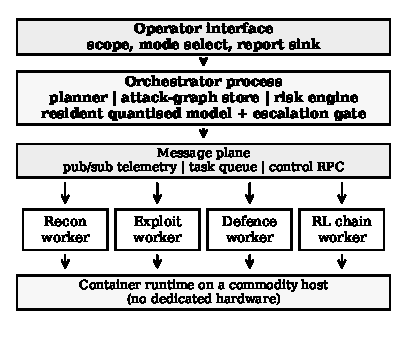
\includegraphics[width=\columnwidth]{fig_architecture}
  \caption{Process architecture. The orchestrator holds the planner, the
           attack-graph store, the risk engine and the resident model. Worker
           processes take typed tasks off the queue and stream results back
           over the message plane. Nothing in the design is specific to a
           particular machine.}
  \label{fig:arch}
\end{figure}

\subsection{Control Plane}

The orchestrator owns the assessment state and every decision that depends on
seeing all of it at once. Concretely it holds the task planner and scheduler
of Equation~(11); the attack-graph store, against which the chain-prediction
agent of Equation~(9) is trained and queried; the retrieval pipeline over
vulnerability and technique catalogues; the risk engine implementing
Equations~(5), (6) and (13); and the resident quantised model together with
the escalation gate of Equation~(10).

Placing scheduling and risk scoring in one process is a deliberate choice
rather than an accident of implementation. Both need a consistent global view
--- the scheduler needs every queue depth, the risk engine needs every
finding --- and splitting either across workers would mean maintaining that
view by consensus, which costs more than the parallelism it would buy at this
scale.

\subsection{Worker Plane}

Workers are single-purpose processes. Each one pulls typed tasks from its
queue, executes them, and publishes results. The reference composition uses
four:

\textbf{Recon worker.} Host and service discovery, banner grabbing, directory
enumeration, and passive fingerprinting over the scoped range. Produces the
raw response of Equation~(2).

\textbf{Exploit worker.} Validation of candidate findings, proof-of-concept
execution against permitted targets, and privilege-escalation path
enumeration. Evaluates Equations~(7) and (8).

\textbf{Defence worker.} Hardening playbooks, patch and configuration
recommendation, rollback testing, and re-assessment of remediated findings.
Drives the remediation term in Equation~(13).

\textbf{Chain worker.} Trains and queries the escalation-prediction agent of
Equation~(9). This worker is optional; the difference it makes is the gap
between configurations B and C throughout Section~VI.

Workers are not pinned to their nominal role. When one queue grows and another
empties, the scheduler of Equation~(11) will hand recon tasks to the exploit
worker, and the queue-variance penalty in that equation exists precisely to
make that reallocation happen before the imbalance becomes expensive.

\subsection{Coordination Model}

Three channels carry different traffic because they have different
requirements. A publish/subscribe topic carries telemetry --- liveness,
progress, resource use --- where loss of an individual message is tolerable. A
durable queue carries task descriptors, where loss is not tolerable and
at-least-once delivery with idempotent task handlers is the right contract. A
request/response channel carries control: start, stop, reconfigure, failover,
priority override. All three are mutually authenticated over TLS.

The cost of this coordination is not free, and we do not treat it as free.
Equation~(12) carries an explicit per-dispatch coordination term measured at
$\gammaC$\,s per worker, and Section~VI-C shows where it starts to dominate.

\subsection{Model-Serving Strategy}

The resident path runs a quantised 4-bit open-weight
model~\cite{touvron2023llama} for routine classification, technique mapping
and report drafting. It executes
on the orchestrator's GPU when one is present and on CPU when it is not, at
reduced throughput but with no change in behaviour.

The escalation path routes to a hosted frontier model when either condition of
Equation~(10) fires: calibrated confidence below $\tauVal$, or accumulated
context beyond the resident window of $\ctxLocal$ tokens. Two Anthropic models
are used as escalation targets, selected for context window and published
price rather than for any benchmark claim we cannot verify: Claude Opus~5
(\texttt{claude-opus-5}, 1M-token context, \$5.00 and \$25.00 per million
input and output tokens) as the default, and Claude Fable~5
(\texttt{claude-fable-5}, 1M-token context, \$10.00 and \$50.00 per million
tokens) for the hardest chain-composition queries~\cite{anthropicmodels}.
Section~VI-E reports what each costs per assessment cycle at the measured
escalation rate.

\subsection{Operational Modes}

In \emph{offensive assessment} mode the operator supplies the scope and the
framework executes the six-phase pipeline of Figure~\ref{fig:pipeline},
looping until the convergence test of Equation~(13) is satisfied or the
iteration budget is exhausted. In \emph{defensive hardening} mode the defence
worker leads: log-driven anomaly identification, detection simulation, and
guided remediation with configuration hardening. The orchestrator's planner is
common to both, which is what makes running them back-to-back on the same
target state cheap.

\begin{figure*}[!t]
  \centering
  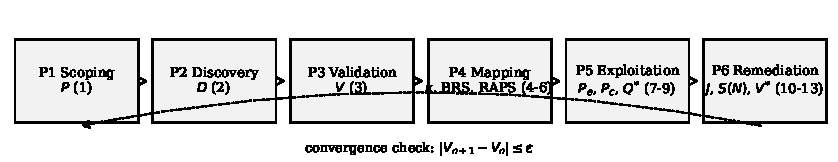
\includegraphics[width=\textwidth]{fig_pipeline}
  \caption{The six-phase assessment cycle and the equations evaluated in each
           phase. The cycle repeats until the change in the active finding
           count falls below $\varepsilon$.}
  \label{fig:pipeline}
\end{figure*}

%=== V. MATHEMATICAL FRAMEWORK =================================================
\section{Mathematical Framework}

At iteration $n$ the assessment tracks a state vector with five components,
$S_n=(V_n, C_n, P_n, R_n, M_n)$, in which $V_n$ is the active
finding set, $C_n$ the set of control-effectiveness values, $P_n$ the
attack-surface index, $R_n$ the composite risk score and $M_n$ the remediation
mass applied in that iteration. Thirteen equations move that state forward.
Each is followed by the value it takes on the testbed of Section~VI-A, so the
framework can be checked rather than taken on trust.

\subsection{Exposure and Discovery}

\textbf{Equation (1): attack-surface index.}
\begin{equation}
  P_n = \frac{E_n \cdot O_n}{T_n}
  \label{eq:surface}
\end{equation}
$E_n$ counts exposed services, $O_n$ reachable paths and $T_n$ enumerated
paths. The product in the numerator is deliberate: a service that is exposed
but unreachable and a path that is reachable but leads nowhere are both
harmless, and only their conjunction is not. On the testbed
$E=\expE$, $O=\expO$ and $T=\expT$, giving $P=\Pindex$.

\textbf{Equation (2): discovery response.}
\begin{equation}
  D_n = \sum_{i} \alpha_i \, s_i + \beta \, g(P_n)
  \label{eq:discovery}
\end{equation}
$\alpha_i \in [0,1]$ is the probability that finding $i$ is detected at the
scan depth the configuration can afford, $s_i$ its indicator, and
$g(P_n)=\log(1+P_n)/\log(1+P_0)$ a normalised topological term weighted by
$\beta$, set to $0.3$ for internal segments and $0.7$ for external-facing
ones. The four-worker configuration yields $D=\Draw$.

\textbf{Equation (3): validated set.}
\begin{equation}
  V_n = D_n\,(1-\mathrm{FPR}) + U_n \cdot \mathrm{FNR}
  \label{eq:validate}
\end{equation}
The raw response is filtered by the measured false-positive rate and credited
with the share of the undetected set $U_n$ that the validation pass recovers.
With the measured $\mathrm{FPR}=\fprC$ and $\mathrm{FNR}=\fnrC$ this gives
$V=\Vval$.

\subsection{Mapping and Prioritisation}

\textbf{Equation (4): technique coverage density.}
\begin{equation}
  \kappa = \frac{1}{|V|}\sum_{i=1}^{|V|}\sum_{j=1}^{m} T_{ij},
  \quad
  T_{ij}=\begin{cases} 1 & j \text{ applies to } i\\
                       0 & \text{otherwise}\end{cases}
  \label{eq:coverage}
\end{equation}
$\kappa$ is the mean number of ATT\&CK techniques a finding maps to, and it is
the quantity that tells an operator whether the mapping stage is doing useful
work or merely labelling. On the testbed $\kappa=\kappaVal$, with all
\techCovered\ of the \techTotal\ techniques in the reference set exercised by
at least one finding --- a mapping density of \mapDensity\,\%.

\textbf{Equation (5): blast-radius score.}
\begin{equation}
  \mathrm{BRS}(v) = \tau_{a(v)} \sum_{k=1}^{5} w_k \, x_k(v)
  \label{eq:brs}
\end{equation}
The five components $x_k$ are confidentiality, integrity and availability
impact, lateral reach and propagation likelihood, with
$w=(0.25,0.25,0.20,0.18,0.12)$. The factor $\tau_{a(v)}$ scales by the
criticality tier of the asset carrying the finding. Mean
$\mathrm{BRS}=\brsMean$, maximum $\brsMax$.

\textbf{Equation (6): risk-adjusted priority.}
\begin{equation}
  \mathrm{RAPS}(v) = a\,P_{\mathrm{exp}}(v) + b\,\mathrm{BRS}(v),
  \quad a=\alphaR,\; b=\betaR
  \label{eq:raps}
\end{equation}
Exploitability and business consequence are separate axes, and a ranking that
uses only one of them will mis-order the queue. The mean RAPS is \rapsMean\
and the top-\topK\ mean is \rapsTop. The practical effect is visible in the
ordering: only \rankOverlap\ of the top \topK\ findings by RAPS are also in
the top \topK\ by severity score alone, a \rankOverlapPct\,\% overlap.

\subsection{Exploitation}

\textbf{Equation (7): single-stage exploitation probability.}
\begin{equation}
  P_{\mathrm{exp}}(v) = \frac{1}{\chi(v)}\bigl(1-\delta(v)\bigr)\,\sigma
  \label{eq:exploit}
\end{equation}
$\chi(v)\in[1,10]$ is attack complexity, $\delta(v)\in[0,1]$ existing defensive
coverage, and $\sigma=\sigmaVal$ a fixed model-assisted skill factor. Holding
$\sigma$ constant is what makes configurations comparable: any difference
between them comes from scheduling and prediction, not from assuming a better
exploiter. Mean $P_{\mathrm{exp}}=\pexpMean$.

\textbf{Equation (8): chain probability.}
\begin{equation}
  P_{\mathrm{chain}}(c) = \prod_{(u,v)\in c}
      P_{\mathrm{exp}}(v)\; P_{\mathrm{esc}}(u \!\to\! v)
  \label{eq:chain}
\end{equation}
Over \nChains\ sampled three-stage chains the mean is $\pchainMean$ with a
95th percentile of $\pchainPnf$. The distribution is the point: chains are
individually unlikely and collectively not, which is why a per-finding screen
under-reports them.

\textbf{Equation (9): chain-prediction value.}
\begin{equation}
  \begin{aligned}
    Q^{*}(s,a) &= \mathbb{E}\bigl[\,r(s,a)
        + \gamma \max_{a'} Q^{*}(s',a')\,\bigr]\\[1pt]
    Q_\theta(s,a) &= \theta^{\!\top}\phi(s,a)
  \end{aligned}
  \label{eq:rl}
\end{equation}
The Bellman optimality condition is standard; the parameterisation is not.
Representing $Q$ as a linear function of edge features
$\phi=(P_{\mathrm{exp}}, 1/\rho, 1-\delta, \mathrm{sev}/10,
\mathbb{1}_{\text{ext}}, \mathrm{BRS}, 1)$ rather than as a table over
$(s,a)$ is what allows a value to be assigned to an escalation edge the agent
never sampled. A table cannot do this, which is the practical reason
tabular treatments of this problem do not generalise past their training
graph. With $\gamma=\gammaQ$ and $\alpha=\alphaQ$ over \episodesQ\ episodes,
$\max Q_\theta = \qstar$.

\subsection{Routing, Scheduling and Convergence}

\textbf{Equation (10): escalation gate and routed cost.}
\begin{equation}
  \begin{aligned}
    \lambda(v) &=
    \begin{cases}
      1, & c(v) < \tau \;\text{ or }\; \eta_{\mathrm{ctx}} > \Omega\\
      0, & \text{otherwise}
    \end{cases}\\[2pt]
    C &= 10^{-6}\sum_{v} \lambda(v)\,
         \bigl(\eta_{i} p_{i} + \eta_{o} p_{o}\bigr)
  \end{aligned}
  \label{eq:route}
\end{equation}
$c(v)$ is calibrated confidence, $\tau=\tauVal$ the gate, $\eta_{\mathrm{ctx}}$
accumulated context against the resident window $\Omega=\ctxLocal$ tokens, and
$(p_i,p_o)$ the published per-million input and output prices of the
escalation target. At $\tau=\tauVal$, \nEsc\ of \numVuln\ findings escalate
(\escFrac\,\%) at a cost of \$\costOpus\ per cycle to Claude Opus~5.

\textbf{Equation (11): task assignment.}
\begin{equation}
  \mathcal{A}(j) = \arg\min_{i}\;
      \bigl[\, L_i \, C_{ij} + \lambda_q \operatorname{Var}(\mathbf{q})
      + q_i \,\bigr]
  \label{eq:assign}
\end{equation}
Task $j$ goes to the worker minimising the product of link latency $L_i$ and
estimated compute cost $C_{ij}$, plus its current backlog $q_i$, plus a
penalty $\lambda_q=\lambdaQ$ on the variance of the queue vector $\mathbf{q}$.
The variance term is what stops the rule from greedily loading the single
fastest worker.

\textbf{Equation (12): speed-up under coordination cost.}
\begin{equation}
  S(N) = \frac{T_1}
   {\,\varsigma T_1 + (1-\varsigma)\dfrac{T_1}{N} + \gamma_c N\,}
  \label{eq:speedup}
\end{equation}
$\varsigma$ is the irreducibly serial share of a cycle, measured at
\serialFrac\,\%, and $\gamma_c=\gammaC$\,s is the per-dispatch coordination
cost. Unlike a pure Amdahl bound, the third term grows with $N$, so $S(N)$ has
a maximum. At $N=4$ the closed form gives $S=\sModelFour$ against a simulated
$\speedupC$; the closed form is the more pessimistic of the two because it
charges the coordination term against every worker rather than against the
dispatches actually made. Measured efficiency at $N=4$ is \effC\,\%.

\textbf{Equation (13): state evolution and equilibrium.}
\begin{align}
  V_{n+1} &= V_n\,(1-\mu_n) + v_{\mathrm{new}},
  & V^{*} &= \frac{v_{\mathrm{new}}}{\mu^{*}} \label{eq:state}\\
  R_{n+1} &= (\rho - \gamma M_n \vartheta)\,R_n + \sigma_r \Sigma_n \nonumber
\end{align}
The active finding count decays by the effective remediation rate
$\mu_n = \eta M_n \vartheta(N)$ and is replenished at $v_{\mathrm{new}}$,
where $\vartheta(N)$ is the throughput factor of $N$ workers. The fixed point
$V^{*}$ is the floor an automated cycle can reach, and it is not zero: with
$\eta=\etaVal$ and $v_{\mathrm{new}}=\vNew$, $V^{*}=\VstarC$ for four workers
against $\VstarA$ for one. The assessment terminates when
$|V_{n+1}-V_n| \le \varepsilon$ with $\varepsilon=\epsConv$.

\subsection{Algorithm}

Algorithm~\ref{alg:cycle} states the loop in the order the implementation
executes it.

\begin{algorithm}[!t]
\caption{PenBox-DMAS assessment cycle}
\label{alg:cycle}
\begin{algorithmic}[1]
\Require scope $\Sigma$, workers $A=\{a_1,\dots,a_N\}$, budget $N_{\max}$,
         tolerance $\varepsilon$
\Ensure  state $S_n$, equilibrium $V^{*}$, report
\State $n \gets 0$; initialise $V_0, C_0, M_0$
\State $P_0 \gets (E_0 O_0)/T_0$ \Comment{Eq.~\eqref{eq:surface}}
\While{$n < N_{\max}$}
  \State dispatch recon tasks by $\mathcal{A}(\cdot)$
         \Comment{Eq.~\eqref{eq:assign}}
  \State $D_n \gets \sum_i \alpha_i s_i + \beta g(P_n)$
         \Comment{Eq.~\eqref{eq:discovery}}
  \State $V_n \gets D_n(1-\mathrm{FPR}) + U_n\mathrm{FNR}$
         \Comment{Eq.~\eqref{eq:validate}}
  \ForAll{$v \in V_n$}
    \State map to techniques; accumulate $\kappa$
           \Comment{Eq.~\eqref{eq:coverage}}
    \State $\mathrm{BRS}(v)$; $\mathrm{RAPS}(v)$
           \Comment{Eqs.~\eqref{eq:brs},~\eqref{eq:raps}}
    \If{$c(v) < \tau$ \textbf{or} $\eta_{\mathrm{ctx}} > \Omega$}
      \State escalate $v$ to the hosted model
             \Comment{Eq.~\eqref{eq:route}}
    \EndIf
  \EndFor
  \State dispatch top-$K$ by RAPS to the exploit worker
  \ForAll{$v$ in top-$K$}
    \State $P_{\mathrm{exp}}(v)$ \Comment{Eq.~\eqref{eq:exploit}}
    \State $P_{\mathrm{chain}}(c)$ for chains through $v$
           \Comment{Eq.~\eqref{eq:chain}}
  \EndFor
  \State query $Q_\theta$ for unseen escalation paths
         \Comment{Eq.~\eqref{eq:rl}}
  \State remediate $\{v : P_{\mathrm{exp}}(v) > \theta_r\}$; update $M_n$
  \State $V_{n+1} \gets V_n(1-\mu_n) + v_{\mathrm{new}}$
         \Comment{Eq.~\eqref{eq:state}}
  \If{$|V_{n+1}-V_n| \le \varepsilon$}
    \State $V^{*} \gets v_{\mathrm{new}}/\mu^{*}$; \textbf{break}
  \EndIf
  \State $n \gets n+1$
\EndWhile
\State \Return $S_n$, $V^{*}$, report
\end{algorithmic}
\end{algorithm}

%=== VI. RESULTS AND DISCUSSIONS ===============================================
\section{Results and Discussions}

\subsection{Experimental Setup}

Everything below comes from an executable model of the framework. There is no
hardware in the loop and no production network was touched. The model consists
of a synthetic target inventory, a discrete-event scheduler that implements
Equation~(11) directly, a chain-prediction agent trained by semi-gradient
Q-learning, and a token-accounting model priced at published list
rates~\cite{anthropicmodels}. One script produces every number and every
figure in this section from seed \seedVal, and the LaTeX source reads that
script's output, so the two cannot disagree.

The inventory spans \numGroups\ target groups, \numHosts\ hosts, \numServices\
services and \numVuln\ ground-truth findings (Table~\ref{tab:testbed}).
Severity scores are drawn per CVSS~v3.1 severity band with the band mix held
fixed across runs; attack complexity is negatively correlated with severity,
so severe findings in this inventory tend to be the easier ones, which is the
conservative direction for the exploitation model of Equation~(7).

\begin{table}[!ht]
  \caption{Synthetic testbed inventory}
  \label{tab:testbed}
  \centering
  \small
  \begin{tabular}{@{}lrrrr@{}}
    \toprule
    \textbf{Group} & \textbf{Hosts} & \textbf{Services}
      & \textbf{Paths} & \textbf{Findings} \\
    \midrule
    Linux-A (ext.)      & 1 & 46 & 38\,/\,74  & 72  \\
    Linux-B (int.)      & 3 & 81 & 59\,/\,132 & 124 \\
    Windows-AD (int.)   & 4 & 63 & 41\,/\,118 & 86  \\
    Embedded/IoT (ext.) & 8 & 37 & 29\,/\,52  & 43  \\
    \midrule
    \textbf{Total} & \textbf{\numHosts} & \textbf{\numServices}
      & \textbf{\expO\,/\,\expT} & \textbf{\numVuln} \\
    \bottomrule
  \end{tabular}
\end{table}

Three configurations are compared throughout. \textbf{Config~A} is the
single-process baseline: one worker, phases in sequence. \textbf{Config~B} is
three concurrent workers without chain prediction. \textbf{Config~C} adds the
fourth worker running the agent of Equation~(9). Detection figures average
\trials\ Monte-Carlo trials; scheduling figures average \reps\ independent
task streams.

\subsection{Detection Performance}

The mechanism that separates the configurations is scan depth. A single
process interleaves scanning with reasoning and reaches \depthA\,\% of the
enumeration budget in the window in which three workers reach \depthB\,\% and
four reach \depthC\,\%. Recall follows: \recA\,\%, \recB\,\% and \recC\,\%
respectively (Table~\ref{tab:confusion}).

\begin{table}[!ht]
  \caption{Classification performance by configuration}
  \label{tab:confusion}
  \centering
  \small
  \begin{tabular}{@{}lrrr@{}}
    \toprule
    \textbf{Metric} & \textbf{Config A} & \textbf{Config B} & \textbf{Config C} \\
    \midrule
    Scan depth achieved & \depthA\,\% & \depthB\,\% & \depthC\,\% \\
    True positives      & \tpA  & \tpB  & \tpC  \\
    False positives     & \fpA  & \fpB  & \fpC  \\
    False negatives     & \fnA  & \fnB  & \fnC  \\
    True negatives      & \tnA  & \tnB  & \tnC  \\
    \midrule
    Recall              & \recA\,\%  & \recB\,\%  & \textbf{\recC\,\%}  \\
    Precision           & \precA\,\% & \precB\,\% & \textbf{\precC\,\%} \\
    Accuracy            & \accA\,\%  & \accB\,\%  & \textbf{\accC\,\%}  \\
    $F_1$               & \foneA     & \foneB     & \textbf{\foneC}     \\
    FPR\,/\,FNR         & \fprA\,/\,\fnrA & \fprB\,/\,\fnrB
                        & \fprC\,/\,\fnrC \\
    \bottomrule
  \end{tabular}
\end{table}

Two things in that table deserve comment rather than celebration. Precision
improves only modestly across configurations (\precA\,\% to \precC\,\%),
because false positives are a function of how much surface is swept and not of
how the sweep is scheduled; parallelism buys recall, not precision. And the
gain from adding the fourth worker (\recB\,\% to \recC\,\%) is roughly a
quarter of the gain from the first three, which is what one should expect once
the depth budget is nearly saturated and the remaining lift comes only from
chain-guided re-scanning.

Per-group results (Table~\ref{tab:groups}, Fig.~\ref{fig:detect}) are
consistent with that reading. The externally-facing groups score highest
(Linux-A at 95.5\,\%, Embedded/IoT at 94.9\,\%) because exposure raises
$\alpha_i$ in Equation~(2) directly. The Windows-AD group is the hardest at
92.7\,\%, which matches its higher share of findings requiring privileged
access.

% generated by dmas_model.py -- do not edit by hand
\begin{table}[!ht]
  \caption{Per-group detection, Config~C}
  \label{tab:groups}
  \centering
  \footnotesize
  \begin{tabular}{@{}lrrrrrc@{}}
    \toprule
    \textbf{Group} & \textbf{Total} & \textbf{Det.} & \textbf{FP} & \textbf{FN} & \textbf{Recall} & \textbf{FPR\,/\,FNR} \\
    \midrule
    Linux-A & 72 & 69 & 4 & 3 & 95.5\% & 0.014\,/\,0.045 \\
    Linux-B & 124 & 114 & 7 & 10 & 91.8\% & 0.014\,/\,0.082 \\
    Windows-AD & 86 & 80 & 5 & 6 & 92.7\% & 0.014\,/\,0.073 \\
    Embedded/IoT & 43 & 41 & 3 & 2 & 94.9\% & 0.014\,/\,0.051 \\
    \midrule
\textbf{Aggregate} & \textbf{325} & \textbf{303} & \textbf{19} & \textbf{22} & \textbf{93.4\%} & \textbf{0.014\,/\,0.066} \\
    \bottomrule
  \end{tabular}
\end{table}


\begin{figure}[!ht]
  \centering
  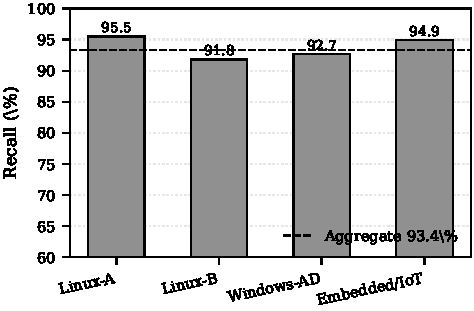
\includegraphics[width=\columnwidth]{fig_detection}
  \caption{Recall by target group for Config~C. The dashed line is the
           aggregate. Externally-facing groups score higher because exposure
           enters $\alpha_i$ directly in Equation~\eqref{eq:discovery}.}
  \label{fig:detect}
\end{figure}

\subsection{Latency and Scaling}

A full cycle of \Tone\,s of accumulated task time completes in
\msA\,$\pm$\,\sdA\,s under Config~A, \msB\,$\pm$\,\sdB\,s under Config~B and
\msC\,$\pm$\,\sdC\,s under Config~C: reductions of \latCutB\,\% and
\latCutC\,\%, or speed-ups of $\speedupB\times$ and $\speedupC\times$.
Figure~\ref{fig:latency} breaks this down by phase.

\begin{figure}[!ht]
  \centering
  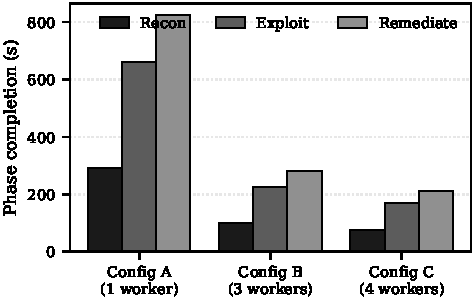
\includegraphics[width=\columnwidth]{fig_latency}
  \caption{Phase completion time by configuration under the assignment rule of
           Equation~\eqref{eq:assign}. The reduction is largest in the exploit
           phase, which holds the longest and most variable tasks.}
  \label{fig:latency}
\end{figure}

Figure~\ref{fig:speedup} sweeps the worker count from one to eight and plots
the measured speed-up against Equation~(12). The two agree closely up to
$N=4$; beyond that the coordination term begins to bite, and the curve reaches
$S=\speedupEight$ at $N=8$ against a linear bound of $8$. Efficiency falls
from \effC\,\% at $N=4$ to \effEight\,\% at $N=8$, while mean worker
utilisation at $N=4$ stays at \utilC\,\% --- the loss is coordination cost,
not idle workers. For an inventory of this size
the useful operating point is four workers, which is where the marginal worker
still returns close to its own throughput.

\begin{figure}[!ht]
  \centering
  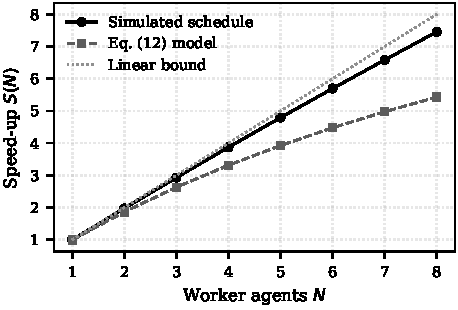
\includegraphics[width=\columnwidth]{fig_speedup}
  \caption{Measured speed-up against Equation~\eqref{eq:speedup} and the
           linear bound. Divergence past $N=4$ is the coordination term
           $\gamma_c N$ rather than queue starvation: mean worker utilisation
           never falls below \utilMin\,\% across the sweep.}
  \label{fig:speedup}
\end{figure}

\subsection{Chain Prediction}

The escalation graph has \nNodesG\ nodes and \totEdges\ edges, of which
\heldOut\ (25\,\%) are withheld during training. Of \nChains\ sampled
three-stage chains, \nUnseen\ traverse at least one withheld edge and
therefore constitute paths the agent has never observed. A chain counts as
viable when its value under Equation~(8) exceeds $\thetaVal$, which puts
\viableFrac\,\% of chains in the positive class. Every method is given the
same treatment: a decision cut-off calibrated for maximum $F_1$ on the seen
chains, then evaluated on the unseen ones.

\begin{table}[!ht]
  \caption{Unseen escalation-chain prediction (\nUnseen\ chains)}
  \label{tab:chain}
  \centering
  \small
  \begin{tabular}{@{}lrrr@{}}
    \toprule
    \textbf{Method} & \textbf{Recall} & \textbf{Precision} & \textbf{$F_1$} \\
    \midrule
    Chain-prediction agent, Eq.~\eqref{eq:rl}
      & \textbf{\rlRate\,\%} & \textbf{\rlPrec\,\%} & \textbf{\rlFone} \\
    Severity-first ranking   & \heurRate\,\% & \heurPrec\,\% & \heurFone \\
    Per-stage screen         & \stageRate\,\% & \stagePrec\,\% & \stageFone \\
    Random control           & \randRate\,\% & \randPrec\,\% & \randFone \\
    \bottomrule
  \end{tabular}
\end{table}

Table~\ref{tab:chain} should be read on $F_1$ and not on recall alone. The
random control reaches \randRate\,\% recall precisely because calibrating a
meaningless score for $F_1$ drives it to label almost everything positive; its
precision of \randPrec\,\% is the base rate, and its $F_1$ of \randFone\ is
the floor. Against that floor the agent scores \rlFone, severity-first ranking
\heurFone\ and the per-stage screen \stageFone.

The per-stage result is the informative one. That screen has the highest
precision of the three baselines (\stagePrec\,\%) and the lowest recall
(\stageRate\,\%), which is exactly the failure mode we predicted in
Section~I-A: judging findings one at a time is reliable when it fires and
silent about most of what matters. Severity-first ranking does better on
recall and worse on precision, because high-severity findings are common
enough that ranking on them alone is only weakly informative about
composability.

Figure~\ref{fig:rl} shows the agent's $F_1$ over training. It passes the
severity-first baseline within roughly 400 episodes and is stable after about
2\,000, and the plateau is the point at which the feature weights stop moving,
not the point at which the graph is exhausted.

\begin{figure}[!ht]
  \centering
  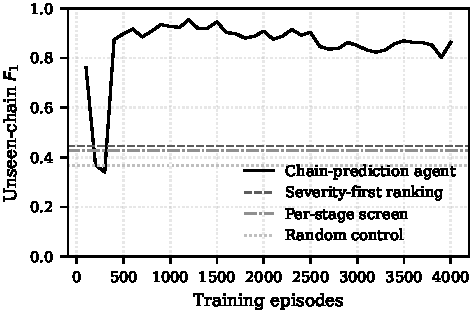
\includegraphics[width=\columnwidth]{fig_rl}
  \caption{Unseen-chain $F_1$ against training episodes, with the three
           baselines as horizontal references. The agent generalises to
           withheld edges because its value function is linear in edge
           features rather than tabular.}
  \label{fig:rl}
\end{figure}

\subsection{Escalation Cost}

At the operating gate $\tau=\tauVal$, \nEsc\ of \numVuln\ findings escalate,
or \escFrac\,\%. Priced at Claude Opus~5's published rate over \tokIn\ input
and \tokOut\ output tokens per escalated finding, that is \$\costOpus\ per
assessment cycle, against \$\costAllOpus\ if every finding were escalated: a
reduction of \costCut\,\%. Routing the same escalated set to Claude Fable~5
costs \$\costFable, exactly double, since its published rate is double.

\begin{table}[!ht]
  \caption{Escalation cost per assessment cycle}
  \label{tab:cost}
  \centering
  \small
  \begin{tabular}{@{}lrrr@{}}
    \toprule
    \textbf{Routing policy} & \textbf{Escalated}
      & \textbf{Cost (USD)} & \textbf{Offline?} \\
    \midrule
    All findings, Opus~5   & \numVuln & \costAllOpus & no  \\
    Resident model only    & 0        & 0.000        & yes \\
    Gated, Opus~5          & \nEsc    & \textbf{\costOpus} & yes \\
    Gated, Fable~5         & \nEsc    & \costFable   & yes \\
    \bottomrule
  \end{tabular}
\end{table}

Figure~\ref{fig:routing} sweeps $\tau$ so the trade-off can be seen rather
than asserted. The escalation share rises roughly linearly with $\tau$ over
the useful range while cost rises with it, and there is no knee: the choice of
$\tau$ is a budget decision, not an optimisation with a natural answer. We
report $\tauVal$ as the operating point because it is where the escalated set
stops growing faster than the number of findings the resident model was
genuinely unsure about, but an operator with a different budget should pick
differently.

\begin{figure}[!ht]
  \centering
  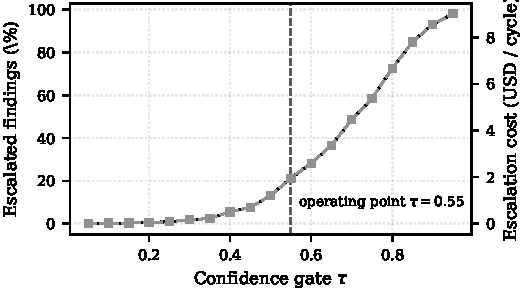
\includegraphics[width=\columnwidth]{fig_routing}
  \caption{Escalated share and per-cycle cost against the confidence gate
           $\tau$ of Equation~\eqref{eq:route}. Costs use published list
           prices for \texttt{claude-opus-5}~\cite{anthropicmodels}.}
  \label{fig:routing}
\end{figure}

\subsection{Prioritisation Behaviour}

Figure~\ref{fig:raps} plots RAPS against severity score, shaded by blast
radius. If prioritisation added nothing, the plot would be a line. It is not:
at any given severity the RAPS spread is wide, and the spread is explained by
blast radius. Only \rankOverlap\ of the top \topK\ findings by RAPS appear in
the top \topK\ by severity alone (\rankOverlapPct\,\%), so slightly more than
half the remediation queue is re-ordered by Equation~(6). Whether that
re-ordering is an improvement is a question this evaluation cannot settle,
because the testbed has no ground truth for business impact; what it can show
is that the two rankings are substantially different, which is the
precondition for the question being worth asking.

\begin{figure}[!ht]
  \centering
  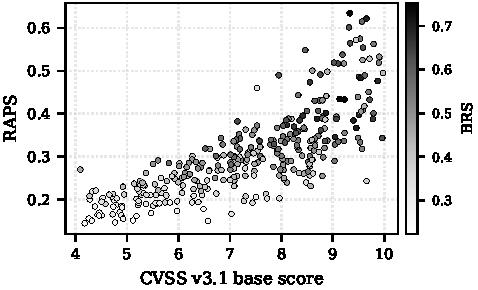
\includegraphics[width=\columnwidth]{fig_raps}
  \caption{RAPS against CVSS~v3.1 base score, shaded by blast-radius score.
           The vertical spread at fixed severity is the contribution of
           Equation~\eqref{eq:brs}.}
  \label{fig:raps}
\end{figure}

\subsection{Convergence}

Figure~\ref{fig:conv} tracks the active finding count and the composite risk
score across iterations. Config~C satisfies $|V_{n+1}-V_n|\le\epsConv$ at
iteration \convC\ against iteration \convA\ for Config~A, a \convCut\,\%
reduction, and settles to $V^{*}=\VstarC$ against $\VstarA$. The risk score
settles to \riskFloorC\ against \riskFloorA.

Neither floor is zero, and that is the result worth keeping. With
$v_{\mathrm{new}}=\vNew$ new findings arriving per iteration and remediation
efficacy $\eta=\etaVal$, Equation~(13) has a strictly positive fixed point.
More workers lower it --- $\mu$ rises from \muA\ to \muC --- but no amount of
parallelism drives it to zero, because the arrival term does not depend on how
many workers are running. An automated cycle converges to a residue; it does
not eliminate one. Any deployment that treats a converged assessment as a
clean assessment has misread what convergence means.

\begin{figure*}[!t]
  \centering
  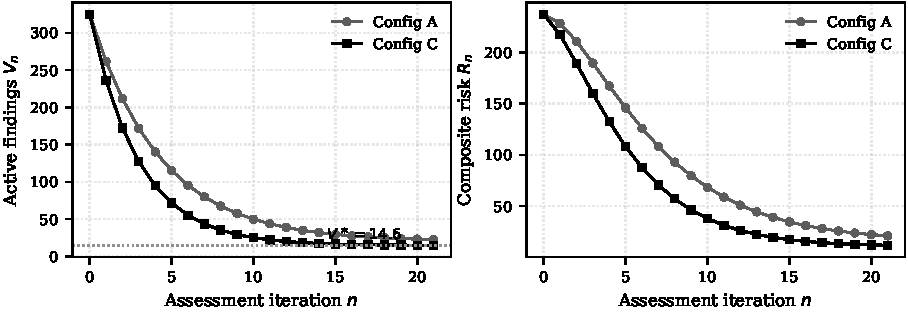
\includegraphics[width=\textwidth]{fig_convergence}
  \caption{Active findings (left) and composite risk (right) across
           iterations. The dotted line marks the equilibrium $V^{*}$ of
           Equation~\eqref{eq:state}. Both configurations converge; they
           converge to different floors, and neither floor is zero.}
  \label{fig:conv}
\end{figure*}

\subsection{Comparison with Prior Systems}

Table~\ref{tab:compare} positions this work against the systems reviewed in
Section~III on capability. We deliberately do not tabulate accuracy figures
across systems. Those numbers were produced on different targets, with
different ground truth and different definitions of a detection, and placing
them in adjacent columns would imply a comparability that does not exist. Two
quantitative results from the literature can be stated as their authors state
them: PentestGPT reports substantial improvement in task completion over a
GPT-3.5 baseline on its own benchmark~\cite{deng2024}, and CHECKMATE reports
improved benchmark success rate together with reduced cost and time per task
relative to prior systems~\cite{deng2024checkmate}. Neither was measured on
the testbed used here, and neither should be read as a comparison against the
numbers in this paper.

\begin{table*}[!t]
  \caption{Capability comparison with prior systems. Accuracy figures are
           deliberately omitted: the systems were evaluated on different
           targets with different ground truth, and tabulating them side by
           side would imply a comparability that does not hold.}
  \label{tab:compare}
  \centering
  \footnotesize
  \begin{tabular}{@{}lcccccc@{}}
    \toprule
    \textbf{Capability}
      & \textbf{PENTEST-AI}~\cite{bianou2024}
      & \textbf{ADAPT}~\cite{skandylas2025}
      & \textbf{CHATIOT}~\cite{dong2025}
      & \textbf{L2M-AID}~\cite{xu2025}
      & \textbf{CHECKMATE}~\cite{deng2024checkmate}
      & \textbf{PenBox-DMAS} \\
    \midrule
    Multi-agent decomposition        & yes & yes & no  & yes & yes & yes \\
    Concurrent phase execution       & no  & no  & no  & no  & no  & \textbf{yes} \\
    Explicit scheduling model        & no  & partial & no & no & no & \textbf{yes}~\eqref{eq:assign} \\
    Multi-stage chain prediction     & no  & no  & no  & yes & no  & \textbf{yes}~\eqref{eq:rl} \\
    Generalises to unseen edges      & no  & no  & no  & no  & no  & \textbf{yes} \\
    Operates with no uplink          & no  & yes & no  & no  & partial & \textbf{yes} \\
    Cost-aware model routing         & no  & no  & no  & no  & yes & \textbf{yes}~\eqref{eq:route} \\
    Convergence-based termination    & no  & no  & no  & no  & no  & \textbf{yes}~\eqref{eq:state} \\
    Integrated remediation loop      & no  & yes & no  & yes & no  & \textbf{yes} \\
    \bottomrule
  \end{tabular}
\end{table*}

\subsection{Consolidated Parameters}

Table~\ref{tab:params} lists every parameter the framework carries, its value
on this testbed, and where it came from. Parameters marked \emph{measured} are
outputs of the model; parameters marked \emph{set} are inputs we chose, and
those are the ones a reader should push on hardest.

\begin{table*}[!t]
  \caption{Parameters, values on the testbed, and provenance}
  \label{tab:params}
  \centering
  \footnotesize
  \begin{tabular}{@{}llllc@{}}
    \toprule
    \textbf{Parameter} & \textbf{Symbol} & \textbf{Meaning}
      & \textbf{Value} & \textbf{Provenance} \\
    \midrule
    Attack-surface index      & $P$         & exposure $\times$ reachability over enumerated paths & \Pindex & measured, Eq.~\eqref{eq:surface} \\
    Topology weight           & $\beta$     & internal / external segment weight & 0.3 / 0.7 & set \\
    False-positive rate       & FPR         & $\mathrm{FP}/(\mathrm{FP}+\mathrm{TN})$ & \fprC & measured, Eq.~\eqref{eq:validate} \\
    False-negative rate       & FNR         & $\mathrm{FN}/(\mathrm{TP}+\mathrm{FN})$ & \fnrC & measured, Eq.~\eqref{eq:validate} \\
    Technique density         & $\kappa$    & mean techniques per finding & \kappaVal & measured, Eq.~\eqref{eq:coverage} \\
    Blast-radius weights      & $w_{1..5}$  & C, I, A, lateral reach, propagation & 0.25, 0.25, 0.20, 0.18, 0.12 & set \\
    Priority mix              & $a$, $b$    & exploitability vs.\ blast radius & \alphaR, \betaR & set \\
    Exploitation skill        & $\sigma$    & model-assisted exploitation factor & \sigmaVal & set, held constant \\
    Escalation probability    & $P_{\mathrm{esc}}$ & mean stage-to-stage transition & \pescVal & set \\
    Discount factor           & $\gamma$    & chain-prediction discount & \gammaQ & set \\
    Learning rate             & $\alpha$    & semi-gradient step size & \alphaQ & set \\
    Confidence gate           & $\tau$      & escalation threshold & \tauVal & set, swept in Fig.~\ref{fig:routing} \\
    Resident context window   & $\Omega$    & local token budget & \ctxLocal & set \\
    Queue-variance penalty    & $\lambda_q$ & load-balancing weight & \lambdaQ & set \\
    Coordination cost         & $\gamma_c$  & seconds per dispatch per worker & \gammaC & measured, Eq.~\eqref{eq:speedup} \\
    Serial share              & $\varsigma$ & non-parallelisable fraction of a cycle & \serialFrac\,\% & measured, Eq.~\eqref{eq:speedup} \\
    Remediation efficacy      & $\eta$      & share of attempted fixes that hold & \etaVal & set \\
    Arrival rate              & $v_{\mathrm{new}}$ & new findings per iteration & \vNew & set \\
    Convergence tolerance     & $\varepsilon$ & termination threshold on $|\Delta V|$ & \epsConv & set \\
    Equilibrium level         & $V^{*}$     & fixed point, 4 workers / 1 worker & \VstarC\ / \VstarA & measured, Eq.~\eqref{eq:state} \\
    \bottomrule
  \end{tabular}
\end{table*}

%=== VII. CONCLUSION ===========================================================
\section{Conclusion and Limitations}

PenBox-DMAS treats a security assessment as a set of concurrent processes
rather than a single pipeline, and this paper gives that treatment a closed
mathematical form: thirteen equations spanning exposure, discovery,
validation, mapping, prioritisation, exploitation, chain prediction, routing,
scheduling and convergence, each evaluated numerically rather than asserted.
On the testbed described, four concurrent workers reach \recC\,\% recall and
\accC\,\% accuracy against \recA\,\% and \accA\,\% for a single-process
baseline, complete a cycle \latCutC\,\% faster, and converge \convCut\,\%
sooner. A chain-prediction agent with a feature-linear value function recovers
\rlRate\,\% of escalation chains withheld from training, where severity-first
ranking recovers \heurRate\,\%. Confidence-gated escalation keeps
\escFrac\,\% of findings off the hosted path and reduces per-cycle escalation
cost by \costCut\,\%.

\subsection{Limitations}

\textbf{The evaluation is a model, not a deployment.} This is the limitation
that bounds every other number in the paper. The results come from an
executable model of the framework running against a synthetic inventory. The
model is reproducible and its assumptions are stated, but a synthetic
inventory cannot reproduce the behaviour of real services under real load, and
none of the reported figures should be read as a measurement of a deployed
system. Field validation is the necessary next step, and until it is done the
right reading of Section~VI is that the architecture is internally consistent
and its trade-offs behave as the equations predict --- not that it performs at
these levels in production.

\textbf{Chain prediction is recombination.} The agent composes known
primitives into sequences absent from the signature set. It does not find new
vulnerability classes. Reported chain-prediction quality is quality on
recombination, and calling it zero-day discovery would be wrong.

\textbf{Parameters we set.} Nine of the parameters in Table~\ref{tab:params}
are inputs, not measurements: the exploitation skill factor $\sigma$, the
blast-radius weights $w_{1..5}$, the priority mix $(a,b)$, remediation
efficacy $\eta$, and the arrival rate $v_{\mathrm{new}}$ among them. Results
that depend heavily on those --- the equilibrium level and the convergence
iteration counts in particular --- inherit their uncertainty. A sensitivity
analysis over them is outstanding work.

\textbf{Escalation is a residual exposure.} Routing to a hosted model sends
metadata off the host. Hashing and transport encryption reduce that exposure;
they do not remove it. Operators with a hard prohibition should disable
escalation and accept the corresponding loss in chain-prediction quality.

\textbf{Scaling was tested to eight workers.} Beyond that the coordination
term of Equation~(12) is extrapolation. The measured optimum on this inventory
is four.

\subsection{Future Work}

\begin{enumerate}
  \item \textbf{Hardware realisation.} The architecture was designed so that
        the control and worker planes could be separated across physical
        machines --- a compute-dense orchestrator node alongside a cluster of
        small single-board workers on a dedicated segment. Nothing in this
        paper is evidence that such a build performs as the software model
        does. The open questions are the ones the model cannot answer: real
        link latency in the coordination term $\gamma_c$, thermal and power
        behaviour under sustained scanning, and recovery when a worker node
        fails mid-cycle rather than mid-task. This is the primary line of
        further work and it needs its own evaluation, not an extrapolation of
        this one.
  \item \textbf{Field validation.} Running the current software framework
        against instrumented live networks with analyst-adjudicated ground
        truth, which is what would let the Section~VI figures be read as
        performance rather than as model behaviour.
  \item \textbf{Sensitivity analysis.} A systematic sweep over the nine set
        parameters, reporting result intervals instead of point values.
  \item \textbf{Federated signature sharing.} Sharing learned chain features
        across deployments without a central collector, so a chain observed at
        one site informs another without either site disclosing its topology.
  \item \textbf{Human adjudication in the loop.} A review step in which a
        qualified tester validates flagged findings and returns corrections
        that retrain the chain-prediction agent, which would close the gap
        between predicted and confirmed exploitability that this evaluation
        currently assumes away.
\end{enumerate}

%=== ACKNOWLEDGEMENT ===========================================================
\section*{Acknowledgement}

The author thanks Dr.~Himanshi Babbar, Department of Computer Science and
Engineering, Chitkara University, for supervision and guidance throughout this
work.

%=== REFERENCES ================================================================
\begin{thebibliography}{99}
\small
\sloppy
\hbadness=10000

\bibitem{sarhaddi2026}
F.~Sarhaddi, N.~T. Nguyen, A.~Zuniga \emph{et al.},
``LLMs and IoT: A comprehensive survey on large language models and the
Internet of Things,''
TechRxiv, Jan.\ 2026,
\doi{10.36227/techrxiv.174063060.01215875/v4}.

\bibitem{skandylas2025}
C.~Skandylas and M.~Asplund,
``Automated penetration testing: Formalization and realization,''
\emph{Computers \& Security}, vol.~155, 2025, Art.\ no.~104454,
\doi{10.1016/j.cose.2025.104454}.

\bibitem{bianou2024}
S.~G. Bianou and R.~G. Batogna,
``PENTEST-AI, an LLM-powered multi-agents framework for penetration testing
automation leveraging MITRE ATT\&CK,''
in \emph{Proc.\ IEEE Int.\ Conf.\ Cyber Security and Resilience (CSR)},
London, U.K., 2024, pp.~763--770,
\doi{10.1109/CSR61664.2024.10679480}.

\bibitem{deng2024}
G.~Deng \emph{et al.},
``PentestGPT: Evaluating and harnessing large language models for automated
penetration testing,''
in \emph{Proc.\ 33rd USENIX Security Symp.}, Philadelphia, PA, USA, Aug.\ 2024.

\bibitem{shen2024}
X.~Shen, L.~Wang, Z.~Li, Y.~Chen, W.~Zhao, D.~Sun, J.~Wang, and W.~Ruan,
``PentestAgent: Incorporating LLM agents to automated penetration testing,''
arXiv:2411.05185, Nov.\ 2024,
\doi{10.48550/arXiv.2411.05185}.

\bibitem{deng2024checkmate}
G.~Deng \emph{et al.},
``Automated penetration testing with LLM agents and classical planning,''
arXiv:2512.11143, Dec.\ 2025,
\doi{10.48550/arXiv.2512.11143}.

\bibitem{yousefi2018}
M.~Yousefi, N.~Mtetwa, Y.~Zhang, and H.~Tianfield,
``A reinforcement learning approach for attack graph analysis,''
in \emph{Proc.\ 17th IEEE Int.\ Conf.\ Trust, Security and Privacy in
Computing and Communications (TrustCom/BigDataSE)}, New York, NY, USA, 2018,
pp.~212--217, \doi{10.1109/TrustCom/BigDataSE.2018.00041}.

\bibitem{sun2025poweriot}
S.~Sun, Y.~Lu, D.~Wu, and G.~Zhang,
``Intelligent penetration testing method for power Internet of Things systems
combining ontology knowledge and reinforcement learning,''
\emph{PLOS ONE}, vol.~20, no.~5, 2025, Art.\ no.~e0323357,
\doi{10.1371/journal.pone.0323357}.

\bibitem{nguyen2025pengym}
H.~P.~T. Nguyen, K.~Hasegawa, K.~Fukushima, and R.~Beuran,
``PenGym: Realistic training environment for reinforcement learning pentesting
agents,''
\emph{Computers \& Security}, vol.~148, 2025, Art.\ no.~104140,
\doi{10.1016/j.cose.2024.104140}.

\bibitem{zhou2025autonomous}
S.~Zhou \emph{et al.},
``Autonomous penetration testing using reinforcement learning: A review and
perspectives,''
\emph{Expert Systems with Applications}, vol.~300, 2025, Art.\ no.~130219,
\doi{10.1016/j.eswa.2025.130219}.

\bibitem{hao2024}
Z.~Hao, H.~Jiang, S.~Jiang, J.~Ren, and T.~Cao,
``Hybrid SLM and LLM for edge-cloud collaborative inference,''
in \emph{Proc.\ Workshop on Edge and Mobile Foundation Models (EdgeFM~'24)},
Tokyo, Japan, 2024, \doi{10.1145/3662006.3662067}.

\bibitem{dong2025}
Y.~Dong, Y.~L. Aung, S.~Chattopadhyay, and J.~Zhou,
``ChatIoT: Large language model-based security assistant for Internet of
Things with retrieval-augmented generation,''
arXiv:2502.09896, Feb.\ 2025,
\doi{10.48550/arXiv.2502.09896}.

\bibitem{xu2025}
T.~Xu, Z.~Wen, X.~Zhao, J.~Wang, Y.~Li, and C.~Liu,
``L2M-AID: Autonomous cyber-physical defense by fusing semantic reasoning of
large language models with multi-agent reinforcement learning,''
arXiv:2510.07363, Oct.\ 2025,
\doi{10.48550/arXiv.2510.07363}.

\bibitem{confido2022}
A.~Confido, E.~V. Ntagiou, and M.~Wallum,
``Reinforcing penetration testing using AI,''
in \emph{Proc.\ IEEE Aerospace Conf.\ (AERO)}, Big Sky, MT, USA, 2022,
pp.~1--15, \doi{10.1109/AERO53065.2022.9843459}.

\bibitem{zhang2025}
J.~Zhang, H.~Bu, H.~Wen, Y.~Liu, H.~Fei, R.~Xi, L.~Li, Y.~Yang, H.~Zhu, and
D.~Meng,
``When LLMs meet cybersecurity: A systematic literature review,''
\emph{Cybersecurity}, vol.~8, no.~1, 2025,
\doi{10.1186/s42400-025-00361-w}.

\bibitem{xu2024survey}
H.~Xu \emph{et al.},
``Large language models for cyber security: A systematic literature review,''
arXiv:2405.04760, May 2024,
\doi{10.48550/arXiv.2405.04760}.

\bibitem{touvron2023llama}
H.~Touvron, T.~Lavril, G.~Izacard \emph{et al.},
``LLaMA: Open and efficient foundation language models,''
arXiv:2302.13971, Feb.\ 2023,
\doi{10.48550/arXiv.2302.13971}.

\bibitem{branescu2024}
I.~Br\u{a}nescu, O.~Grigorescu, and M.~Dasc\u{a}lu,
``Automated mapping of common vulnerabilities and exposures to MITRE ATT\&CK
tactics,''
\emph{Information}, vol.~15, no.~4, 2024, Art.\ no.~214,
\doi{10.3390/info15040214}.

\bibitem{zong2025}
M.~Zong, A.~Hekmati, M.~Guastalla, Y.~Li, and B.~Krishnamachari,
``Integrating large language models with Internet of Things: Applications,''
\emph{Discover Internet of Things}, vol.~5, no.~2, 2025,
\doi{10.1007/s43926-024-00083-4}.

\bibitem{anthropicmodels}
Anthropic, ``Models overview --- context windows and pricing,'' Anthropic
developer documentation. [Online].
Available: \url{https://platform.claude.com/docs/en/about-claude/models/overview}.
Accessed: Aug.~2, 2026.

\end{thebibliography}

\end{document}
